\title{The Graph Hessian}

Everybody knows about the graph Laplacian, but can we define the Hessian
operator on a graph?  Let us see.

\section{Recall of algebraic graph calculus}

Consider a directed graph~$G=(V,E)$ with~$n$ vertices and~$m$ edges.

\newcommand{\R}{\mathbf{R}}
\newcommand{\Z}{\mathbf{Z}}
\newcommand{\diag}[1]{\,\mathrm{d}\!\left(#1\right)}

Functions~$f:V\to\R$ are called~\emph{scalar fields}
and they are elements of~$\R^n$.

Functions~$X:E\to\R$ are called~\emph{vector fields} and they are elements
of~$\R^m$.  For an intuition, you may think that the values of~$X$ on the
edges around a vertex~$p\in V$ are the components of the vector~$X_p$.


The~\emph{signed incidence matrix}~$B$ has~$m$ rows and~$n$ columns, encoding
the directed edges with~$\pm 1$.  More precisely, if~$e=(i,j)\in E$ this
means that~$B_{ei}=-1$, $B_{ej}=1$ and zero elsewhere.  The linear
operator~$B:\R^n\to\R^m$ transforms scalar fields into vector fields and is
called the~\emph{gradient}.  Given a scalar field~$f:V\to\R$, its gradient is
a vector field that at each edge~$e=(i,j)\in E$ takes the value~$f(j)-f(i)$.

The linear operator~$-B^\top:\R^m\to\R^n$ transforms vector fields into
scalar fields and is called the~\emph{divergence}.  Given a vector
field~$X:E\to\R$ its divergence is a scalar field that represents the
difference between the inflow and outflow at each vertex.

The~\emph{laplacian} is the divergence of the gradient~$L=-B^\top B$.  As
an~$n\times n$ matrix, it is symmetric and negative semidefinite.  As a
linear operator, it transforms scalar fields into scalar fields.  The
condition~$Lf=0$ for a scalar field~$f$ is an equilibrium condition:
the value of~$f$ at one vertex is equal to the average value on all its
neighbours.

These definitions are analogous to the corresponding constructions of vector
calculus in~$\R^2$ and~$\R^3$.  However, not all operations that we can do in
vector calculus are possible here.  For example, the pointwise product of a
scalar and a vector field is not well defined in the discrete case.  For that
we'll need to introduce a specific~\emph{centering
operator} defined by~$C=\frac12\left|B\right|$.

The centering operator~$C:\R^n\to\R^m$ transforms scalar fields into vector
fields, just like the gradient; but it takes the average instead of the
difference at each edge. Similarly, the operator~$C^\top$ takes vector fields
into scalar fields.

Thanks to the centering operator we can prove the discrete analogs of the
traditional product rules from vector calculus
\begin{equation}\label{eq:vectorcalculus}
	\nabla\left(fg\right)=f\nabla g+g\nabla f
	\qquad
	\qquad
	\mathrm{div}\left(fX\right)
	=f\mathrm{div}X+X\cdot\nabla f
\end{equation}

In the discrete case, to avoid algebraic confusion,
we will denote pointwise products in~$\R^d$
by~$\odot_d$.  Thus the pointwise product of two scalar fields~$f$ and~$g$ is
the scalar field~$f\odot_n g$.  We also define the product of a scalar
field~$f$ with a vector field~$X$ as the vector field~$Cf\odot_m X$, and the
dot product of two vector fields~$X$ and~$Y$ as the scalar
field~$C^\top\left(X\odot_m Y\right)$.


We readily check the product rule for the discrete gradient:
\begin{equation}\label{eq:gradprod}
	B\left(f\odot_n g\right)=
	Cf\odot_m Bg + Bf\odot_m Cg
\end{equation}
and, with some more work, the product rule for the divergence
\begin{equation}\label{eq:divprod}
	-B^\top\left(Cf\odot_m X\right)
	=
	f\odot_n\left(-B^\top X\right)
	+C^\top\left(X\odot_m Bf\right)
\end{equation}
Notice that formulas~\eqref{eq:gradprod} and~\eqref{eq:divprod} may appear
complicated at first sight, but they are the exact translation of the
traditional product rules~\eqref{eq:vectorcalculus}.  You don't need to
remember these complicated formulas: you deduce them every time you need, by
writing the traditional product rule and adding centering operators until the
dimensions fit.

{\color{gray}
An interesting particular case of these computations is when~$G$ is the
one-dimensional path graph.  For example let~$V=\Z$ with edges joining
consecutive integers from low to high.  Now, if~$f:\Z\to\R$ is a discrete
function, the gradient~$Bf$ is the discrete derivative computed by forward
differences (which is defined at half-positions, that is, on the edges!).
The operator~$-B^\top$ is backwards finite differences, and composing both we
obtain the second derivative~$L f$ by the traditional three-point scheme:
\[
	Lf (i) = f(i-1) -2f(i)+f(i+1)
\]
Using the traditional (but confusing) notation for finite
differences~$\Delta_1 f(i)=f(i+1)-f(i)$, we can rewrite the
formula~\eqref{eq:gradprod} as
\[
	\Delta_1(fg)(i) =
	\tfrac{f(i)+f(i+1)}2\Delta_1 g(i) +
	\tfrac{g(i)+g(i+1)}2\Delta_1 f(i)
\]
which is the most natural form of the product rule for discrete derivatives
(exact, and with only two terms, unlike some horrendous monstrosities that
are often found in numerical analysis books).  Here we see that the centering
operator is necessary, but it arises in a natural way.
}

Finally, as a sanity check, we can verify the
product rule for the Laplacian:~$\Delta\left(fg\right)=f\Delta g+g\Delta
f+2\nabla f\cdot\nabla g$:
\[
	L\left(fg\right)=
	f\odot_n Lg
	+
	g\odot_n Lf
	+2C^\top\left(Bf\odot_m Bg\right)
\]
This follows directly by applying equations~\eqref{eq:gradprod}
and~\eqref{eq:divprod} one after the other.

By analogy with the continuous case, we define the \emph{directional
derivative} of a function~$f$ with respect to a vector field~$X$
as~$\partial_Xf:=C^\top\left(X\odot_m Bf\right)$.  Notice that this is just a
linear operator (depending on~$X$) applied to~$f$.  Indeed, if we denote
by~$d(X)$ the~$m\times m$ matrix with the elements of~$X$ at the diagonal, we
see that~$X\odot_m Y=d(X)Y$, thus the matrix of the operator~$\partial_X$
is~$C^\top d(X)B$.  Furthermore, the map~$X\mapsto\partial_Xf$ is also linear
on~$X$, and its matrix is~$C^\top d\left(Bf\right)$.  These observations will
be crucial when we try to define the Hessian as a bilinear operator.


\section{Definition of the Hessian}

In differential geometry, the Hessian is a second-order symmetric tensor that
is defined on a Riemannian manifold.  The Riemannian structure is either
given by a metric tensor~$g$ or by a torsion-free connection~$\nabla$.  The
Hessian of a function~$f$ will thus be a symmetric bilinear form that takes
two vector fields~$X$, $Y$ and returns a
function~$\mathrm{Hess}\left(f\right)\left(X,Y\right)$.  See e.g. Jost's book
\emph{Riemannian Geometry and Geometric Analysis} for a list of equivalent
definitions.

\[
	\mathrm{Hess}\left(f\right)\left(X,Y\right)
	=
	g\left(\nabla_X\,\mathrm{grad}f,Y\right)
\]
\[
	\mathrm{Hess}\left(f\right)\left(X,Y\right)
	=
	X\left(Y\left(f\right)\right)-\left(\nabla_X Y\right)f
	=
	X\left(Y\left(f\right)\right)-\mathrm{d}f\left(\nabla_X Y\right)
\]
\[
	\mathrm{Hess}\left(f\right)
	=
	\nabla\nabla f
	=\nabla \mathrm{d} f
\]
\[
	\mathrm{Hess}\left(f\right)
	=
	\frac12L_{\nabla f} \left(g\right)
\]

None of these general definitions is easily adaptable to the discrete
setting, for we have not defined the discrete connection.  But there is a
beautiful property: the Hessian at a critical point~$p$ of~$f$ does not depend
on the metric, but it is a 2-tensor at~$p$ that can be defined
intrinsically:~$\mathrm{Hess}_p\left(f\right)(X,Y)=
X_p\left(Y\left(f\right)\right)$.  This property does not seem to lead to
any definition, but we may use it later as a sort of sanity check.

A first attempt at defining a discrete Hessian may look something like this:
\[
	\mathrm{Hess}\left(f\right)(X,Y)
	\quad
	:=
	\quad
	C^\top\left(\left(BC^\top Bf\right)\odot X\odot Y\right)
\]
at first sight, it seems to work: it is a scalar field, it is linear
on~$f$,~$X$ and~$Y$, it is symmetric on~$(X,Y)$, the scalar field is differentiated twice with the direct
derivative (not the adjoint), neither~$X$ nor~$Y$ are differentiated.
But this formula cannot be correct.  For example, when the graph is a 2D
grid, and the fields~$X$,$Y$ are the coordinate axis (or any perpendicular
fields), this expression gives zero, but it should give something
related to~$f_{xy}$.

Thinking about this case, we may impose that it works at least for the 2D
grid, using vector coordinate fields~$X=\frac{\partial}{\partial x}$, etc.
Thus, it seems that if the fields $X,Y$ commute (e.g., they are equal, or
orthogonal), we should have
\[
	H(f)(X,Y):= \partial_Y(\partial_X(f)) =\partial_Y(C^\top(X\odot Bf))
	=C^\top(Y\odot B(C^\top(X\odot Bf)))
\]
This is actually a good first start; it has all the nice properties except
symmetry between~$X$ and~$Y$.

We can impose symmetry into this expression by taking the average of both
cases:
\begin{equation*}
	H(f)(X,Y):=
	\frac{
		C^\top(Y\odot B(C^\top(X\odot Bf)))
		+
		C^\top(X\odot B(C^\top(Y\odot Bf)))
	}2
\end{equation*}
which, after some arrangement becomes
\begin{equation}\label{eq:badhessian}
	H(f)(X,Y):=
	C^\top\left(
		\frac{
			\diag{Y}BC^\top\diag{X}
			+
			\diag{X}BC^\top\diag{Y}
		}2
	\right) Bf
\end{equation}
which is a good start.  We will check later how bad this is numerically.

Unfortunately, formula~\eqref{eq:badhessian} cannot be right.  It continuous
version is a sort of Lie Bracket with a plus sign, which is
definitely~\emph{not} the Hessian, even in Euclidan space.
Even worse, it is a vector field (defined by the expression inside
parentheses) acting over the function~$f$, which cannot be the Hessian in any
meaningful way.  In the continuous setting that would mean that for every two
fields~$X,Y$ there exists a field~$Z$ such that~$H(u)(X,Y)=Z\cdot\nabla u$

A way out is given by the famous Koszul formula, that expresses the covariant
derivative in terms of the metric. Koszul formula can then be combined with
the first formula above to yield a purely intrinsic definition of the Hessian
that does not depend on the connection, only on the metric.
%: \emph{(unwyeldy expression follows)}

Recall Koszul formula in Riemannian geometry:
\[
	\begin{array}{ll}
		2 g(\nabla_XY, Z) &=
		X g(Y,Z)
		+
		Y g(X,Z)
		-
		Z g(X,Y) \\
		&
		\quad + g([X,Y],Z) - g([X,Z],Y) - g([Y,Z],X)
	\end{array}
\]
where~$g$ denotes the metric,~$Xu$ denotes~$\partial_X u$ and~$\nabla_XY$ is
the connection.  This formula defines the metric connection in terms of the
metric, by applying it to arbitrary fields~$Z$ we can completely
recover~$\nabla_XY$.  Thus, we can remove the connection from any definition
in which it appears.  In particular from~$H(u)(X,Y)=g(\nabla_X\,\mathrm{grad}
f,\,Y)$.  Thus we obtain the following expression for the Hessian
\begin{equation*}
	\mathrm{Hess}\left(f\right)(X,Y) =
	\frac12\left(
		\begin{array}{l}
		X g\!\left(\mathrm{grad}\!\left(f\right),Y\right)\\
		+
		\mathrm{grad}\!\left(f\right) g\!\left(X,Y\right)\\
		-
		Y g\!\left(X,\mathrm{grad}\!\left(f\right)\right) \\
		+
		g\!\left(\left[X,\,\mathrm{grad}\!\left(f\right)\right],Y\right)\\
		-
		g\!\left(\left[X,\,Y\right],\,\mathrm{grad}\!\left(f\right)\right)\\
		-
		g\!\left(\left[\mathrm{grad}\!\left(f\right),\,Y\right],X\right)
		\end{array}
	\right)
\end{equation*}
(sum of the six terms inside the parenthesis).  Now we can use this
expression as definition of the Hessian in terms of objects that have a
correspondence in the discrete setting (see the Rosetta stone at the
end).  The following ``translation'' into the discrete setting is automatic:
\begin{equation*}
	\mathrm{Hess}\left(f\right)(X,Y) :=
	\frac12\left(
		\begin{array}{l}
		%X g\!\left(\mathrm{grad}\!\left(f\right),Y\right)
		C^\top\left(X\odot\left(BC^\top\left(Y\odot Bf\right)\right)\right)
		\\
		+
		%\mathrm{grad}\!\left(f\right) g\!\left(X,Y\right)
		C^\top\left(\left( Bf \right)\odot BC^\top\left(X\odot Y\right)\right)
		\\
		-
		%Y g\!\left(X,\mathrm{grad}\!\left(f\right)\right)
		C^\top\left(Y\odot\left(BC^\top\left(X\odot Bf\right)\right)\right)
		\\
		+
		%g\!\left(\left[X,\,\mathrm{grad}\!\left(f\right)\right],Y\right)
		%C^\top\left(\left([X,Bf]) \right)\odot Y\right)
		C^\top\left(\left(
				% [X,Bf]
				\diag{X}BC^\top Bf-\diag{Bf}BC^\top X
		) \right)\odot Y\right)
		\\
		-
		%g\!\left(\left[X,\,Y\right],\,\mathrm{grad}\!\left(f\right)\right)
		%C^\top\left([X,Y]\odot Bf\right)
		C^\top\left(
			%[X,Y]
			\left(
				\diag{X}BC^\top Y-\diag{Y}BC^\top X
			\right)
			\odot Bf\right)
		\\
		-
		%g\!\left(\left[\mathrm{grad}\!\left(f\right),\,Y\right],X\right)
		%C^\top\left( [Bf\odot Y]\odot X \right)
		C^\top\left(
			\left(
				%[Bf\odot Y]
				\diag{Bf}BC^\top Y-\diag{Y}BC^\top Bf
			\right)
		\odot X \right)
		\end{array}
	\right)
\end{equation*}
We will try to simplify this formidable expression, but first note that it
has a few desirable properties:  it is linear with respect to~$X$,~$Y$
and~$f$; the function~$f$ is differentiated twice; the role of~$X$ and~$Y$ is
symmetrical (as~$X$ and~$Z$ are in the original Koszul formula); and,
interestingly, it is not obviously a vector field acting on~$f$, although
four of the six terms are.

We can rewrite the terms by trying to put~$Bf$ towards the end, as much as
possible, and developing~$F\odot G$ as~$\diag{F}G$:
\begin{equation*}
	\mathrm{Hess}\left(f\right)(X,Y) :=
	\frac12C^\top\left(
		\begin{array}{l}
			\diag{X}BC^T\diag{Y}Bf\\
			+{\color{Green4}\diag{BC^\top\diag{X}Y}}Bf\\
			-\diag{Y}BC^\top\diag{X}Bf\\
			+\diag{Y}\diag{X}BC^\top Bf\\
			-\diag{Y}{\color{red}\diag{Bf}}BC^\top X\\
			-{\color{blue}\diag{\diag{X}BC^\top Y}}Bf\\
			+{\color{blue}\diag{\diag{Y}BC^\top X}}Bf\\
			-\diag{X}{\color{red}\diag{Bf}}BC^\top Y\\
			+\diag{X}\diag{Y}BC^\top Bf
		\end{array}
	\right)
\end{equation*}
and rearranging the terms (not sure this is the most reasonable way):
\begin{equation*}
	\begin{array}{lll}
		\mathrm{Hess}\left(f\right)(X,Y) & :=
		C^\top\diag{X}\diag{Y}BC^\top Bf &{\color{gray}
		\small(T1)}\\
		&\quad +C^\top\frac{\diag{X}BC^T\diag{Y}-\diag{Y}BC^\top\diag{X}}2Bf &{\color{gray}
		\small(T2)}\\
		&\quad +C^\top{\color{blue}\diag{\frac{
			{\diag{Y}BC^\top X}-\diag{X}BC^\top Y}2
	}}Bf &{\color{gray}
	\small(T3)}\\
		&\quad -C^\top\frac{\diag{Y}{\color{red}\diag{Bf}}BC^\top X
			+\diag{X}{\color{red}\diag{Bf}}BC^\top Y
		}2 &{\color{gray}
		\small(T4)}\\
		&\quad +\frac12 C^\top{\color{Green4}\diag{BC^\top\diag{X}Y}}Bf &{\color{gray}
		\small(T5)}\\
	\end{array}
\end{equation*}
We can sort of interpret each of these five terms.  The first term~$(T1)$ is
the original bad definition we gave of the Hessian as~$C^\top(X\odot Y\odot
BC^\top Bf)$.  Nice to see it appear naturally here.
%The second term~$(T2)$ is the second bad definition that we proposed, as a
%sort of Lie bracket with positive sign.
The third term~$(T3)$ is simply~$\partial_{[X,Y]} f$.  The
fourth term~$(T4)$ is the only term that is not the action by a vector field
over~$f$ (or equivalently, the effect of applying the differential
form~$\mathrm{d}u$ over a vector field).  Finally, we recognize the last
term~$(T5)$ as~$\frac12\partial_{\mathrm{grad}\left(X\boldsymbol{\cdot}
Y\right)}f=\frac12\partial_{\mathrm{grad} f}\,\left(X\boldsymbol{\cdot}
Y\right)$, as it appears in the original Koszul formula.
It seems as if terms~$(T2)$ and~$(T3)$ should cancel each other, but I'm not
sure.

In the following section we study the numerical effect of each of these
terms, and their ``impulse response'' when the graph is a regular grid.

\clearpage
\section{Numerical verification}

None of this would be any good if it wasn't easy to verify numerically.  Let
us check whether all these derivatives make sense for a 2D image.  I do these
experiments because the formulas that we'll find later for the Hessian will
be so scary that we'll need to verify them...

Let us consider a~$128\times128$ image with a Gaussian profile, together with
some of its derivatives


\begin{tabular}{cccccc}

\includegraphics{fgauss.png} &

\includegraphics{fgaussx.png} &

\includegraphics{fgaussy.png} &
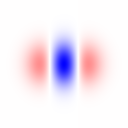
\includegraphics{fgaussxx.png} &

\includegraphics{fgaussxy.png} &
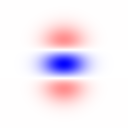
\includegraphics{fgaussyy.png} \\
$u$ & $u_x$ & $u_y$ & $u_{xx}$ & $u_{xy}$ & $u_{yy}$
\end{tabular}
%SCRIPT plambda zero:128x128 ":r 2 ^ -0.1 / exp" -o fgauss.npy
%SCRIPT palette {-,}1 nice fgauss.npy fgauss.png
%SCRIPT plambda fgauss.npy "u,x"|palette {-,}0.05 nice - fgaussx.png
%SCRIPT plambda fgauss.npy "u,y"|palette {-,}0.05 nice - fgaussy.png
%SCRIPT plambda fgauss.npy "u,xx"|palette {-,}0.005 nice - fgaussxx.png
%SCRIPT plambda fgauss.npy "u,xy"|palette {-,}0.005 nice - fgaussxy.png
%SCRIPT plambda fgauss.npy "u,yy"|palette {-,}0.005 nice - fgaussyy.png
%SCRIPT plambda fgauss.npy "u,g"|viewflow 0.05 - fgaussg.png
%SCRIPT plambda fgauss.npy "u,n"|palette {-,}0.08 nice - fgaussgn.png
%SCRIPT plambda fgauss.npy "u,l"|palette {-,}0.005 nice - fgaussl.png
%SCRIPT plambda fgauss.npy "u,xx u,yy * u,xy 2 ^ -"|palette {-,}0.00004 nice - fgaussd.png
%SCRIPT plambda fgauss.npy "u,xx u,x 2 ^ * u,yy u,y 2 ^ * u,xy u,x u,y * * -2 * + +"|palette {-,}0.000005 nice - fgaussc.png
%SCRIPT plambda fgauss.npy "u,g dup vnorm /"|plambda "u,d -1 *"|palette {-,}1 nice - fgaussk.png

\bigskip

\begin{tabular}{cccccc}

\includegraphics{fgaussgn.png} &

\includegraphics{fgaussg.png} &

\includegraphics{fgaussl.png} &

\includegraphics{fgaussd.png} &

\includegraphics{fgaussc.png} &
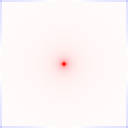
\includegraphics{fgaussk.png} \\
$\left\|\nabla u\right\|$ &
$\mathrm{vec}\left(\nabla u\right)$ &
$\Delta u$ &
$\mathrm{det}H u$ &
$\mathrm{canny}(u)$ &
$\mathrm{curv}(u)$
\end{tabular}

For reference, these images have been produced using the following shell
script
% do not remove the space before verbatim
 \begin{verbatim}
plambda zero:128x128 ":r 2 ^ -0.1 / exp" -o fgauss.npy
palette {-,}1 nice fgauss.npy fgauss.png
plambda fgauss.npy "u,x"  | palette {-,}0.05  nice - fgaussx.png
plambda fgauss.npy "u,y"  | palette {-,}0.05  nice - fgaussy.png
plambda fgauss.npy "u,xx" | palette {-,}0.005 nice - fgaussxx.png
plambda fgauss.npy "u,xy" | palette {-,}0.005 nice - fgaussxy.png
plambda fgauss.npy "u,yy" | palette {-,}0.005 nice - fgaussyy.png
\end{verbatim}% do not remove this comment


All these computations have been performed using classical finite difference
schemes.  Now, let us verify that the computations using the graph
formalism give the same results.  The rest of the code shown is written in
Octave.

%RUN_VERBATIMS octavescript

First, we define the only ``structural'' function that we will need, to
compute the signed incidence matrix of a rectangular grid:

\begin{verbatim}
function B = grid_incidence(w, h)                          # grid graph WxH
        x = sparse(1:w-1, 2:w, 1, w-1, w) - speye(w-1,w);  # path of length W
        y = sparse(1:h-1, 2:h, 1, h-1, h) - speye(h-1,h);  # path of length H
        B = [ kron(speye(h),x) ; kron(y,speye(w)) ];       # kronecker union
end
\end{verbatim}

Now we are good to go.  Let us start by loading the image data and defining
all the appropriate matrices:

\begin{verbatim}
u = iio_read("fgauss.npy");   # load input image
[w,h] = size(u);              # extract dimensions
u = double(u(:));             # flatten image data into vector
B = grid_incidence(w,h);      # build incidence matrix
C = abs(B)/2;                 # centering matrix
L = -B'*B;                    # laplacian matrix
\end{verbatim}

As a first test, we will compute and visualize the laplacian of this image:
\begin{verbatim}
v = L*u;                                     # compute the laplacian
z = 127 + 127*v/max(abs(v));                 # normalize values into [0,255]
iio_write("fgauss_Lu.png", reshape(z,w,h));  # save the result
\end{verbatim}


\includegraphics{fgauss_Lu.png}\verb+ fgauss_Lu.png+

So far, it looks good.  Since at this point we only have one function~$u$,
and we can only visualize scalar fields, maybe the easiest numerical check
will be to verify the formula
\[
	\mathrm{div}\left(u\nabla u\right) = u\Delta u+\left\|\nabla
	u\right\|^2
\]
or, in the discrete case
\[
	-B^\top\left(Cf\odot_mBf\right)
	=
	f\odot_n\left(-B^\top B f\right)
	+C^\top\left(Bf\odot_mBf\right)
\]
and, in code
\begin{verbatim}
a = -B' * ( (C*u) .* (B*u) );   # f = div(u*grad(u))
b = u .* (-B'*B*u);             # g = u*lap(u)
c = C' * ( (B*u) .* (B*u) );    # h = |grad(u)|^2
bpc = b + c;
err = a - bpc;

na = 127 + 127*a/max(abs(a));
nb = 127 + 127*b/max(abs(b));
nc = 127 + 127*c/max(abs(c));
nbpc = 127 + 127*bpc/max(abs(bpc));
nerr = 127 + 127*err/max(abs(err));

iio_write("fgauss_a.png", reshape(na,w,h));
iio_write("fgauss_b.png", reshape(nb,w,h));
iio_write("fgauss_c.png", reshape(nc,w,h));
iio_write("fgauss_bpc.png", reshape(nbpc,w,h));
iio_write("fgauss_err.png", reshape(nerr,w,h));
iio_write("fgauss_err.npy", reshape(err,w,h));
\end{verbatim}

\begin{tabular}{ccccc}
	
\includegraphics{fgauss_a.png} &
	
\includegraphics{fgauss_b.png} &
	
\includegraphics{fgauss_c.png} &
	
\includegraphics{fgauss_bpc.png} &
	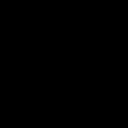
\includegraphics{fgauss_err.png}\\
	$a$ &
	$b$ &
	$c$ &
	$b+c$ &
	$a-(b+c)$
\end{tabular}

The product rule is uncannily precise!


Now let us compute some directional derivatives.

\begin{verbatim}
[x,y] = meshgrid(linspace(1,w,w),linspace(1,h,h));
Dx = B*x(:);
Dy = B*y(:);
ux = C'*( Dx .* (B*u) );
uy = C'*( Dy .* (B*u) );
nux = 127 + 127*ux/max(abs(ux));
nuy = 127 + 127*uy/max(abs(uy));
iio_write("fgauss_ux.png", reshape(nux,w,h));
iio_write("fgauss_uy.png", reshape(nuy,w,h));
\end{verbatim}


\includegraphics{fgauss_ux.png}\verb+ fgauss_ux.png+


\includegraphics{fgauss_uy.png}\verb+ fgauss_uy.png+


Let us check whether~$\partial_X$ is a derivation.  In the continuous case
this property is
\[
	\partial_X\left(fg\right)
	=
	f\partial_X\left(g\right)
	+
	g\partial_X\left(f\right)
\]
and for a graph this reads
\[
	C^\top d(X)B\left(f\odot_n g\right)
	f\odot :wqC^\top d(X)
\]

\clearpage
\section{$\mathfrak{der\ Rosettastein}$}

Objects:\newline
\begin{tabular}{|l|l|}
	\hline
	{\bf Continuous} & {\bf Discrete} \\
	\hline
	manifold $M=\R^2$ or $M=\R^3$ & graph $G=(V,E)$ \\
	\hline
	point~$p\in M$ & vertex~$p\in V$ \\
	\hline
	tangent vector~$X_p\in T_pM$ & edge~$(p,q)\in E$ \\
	\hline
	set of all points~$M$ & $V=\{1,\ldots,n\}$ \\
	\hline
	tangent bundle~$TM$ & $E=\{1,\ldots,m\}$ \\
	\hline
	function~$f:M\to\R$ & function~$f:V\to\R$ \\
	& $f\in\R^n$ \\
	\hline
	(co)vector field~$X$ & function~$X:E\to\R$ \\
	& $X\in\R^m$ \\
	\hline
	set of all functions~$\mathcal{C}^\infty(M)$ & $\R^n$ \\
	\hline
	set of all vector fields~$\mathfrak{X}(M)$ & $\R^m$ \\
	\hline
\end{tabular}

\bigskip




Differential calculus:\newline
\begin{tabular}{|l|l|l}
	\cline{1-2}
	{\bf Continuous} & {\bf Discrete} &\\
	\cline{1-2}
		%gradient~
	$\nabla:\mathcal{C}^\infty(M)\to\mathfrak{X}(M)$ & signed incidence
		%matrix~$B\in\mathcal{M}_{m,n}(\R)$ &\\
	matrix~$B:\R^n\to\R^m$ &\\
	\cline{1-2}
	?%\emph{(nothing)}
	& centering matrix~$C=\tfrac12|B|$ &\\
	\cline{1-2}
		%divergence~
	$\mathrm{div}:\mathfrak{X}(M)\to\mathcal{C}^\infty(M)$
	& $-B^\top:\R^m\to\R^n$ &\\
	\cline{1-2}
	$\Delta:\mathcal{C}^\infty(M)\to\mathcal{C}^\infty(M)$ &
	$L=-B^\top B : \R^n\to\R^n$ &\\
	\cline{1-2}
	$fg$ & $f\odot g\quad$
	%{\small\color{gray}(component-wise product in~$\R^n$)}
	& {\small $(D1)$}\\
	& $\color{gray}\diag{f}g$ & \\
	& $\color{gray}\diag{g}f$ & \\
	\cline{1-2}
	$fX$ & $X\odot Cf\quad$
	%{\small\color{gray}(component-wise product in~$\R^m$)}
	&{\small $(D2)$} \\
	& $\color{gray}\diag{X}Cf$ & \\
	& $\color{gray}\diag{Cf}X$ & \\
	\cline{1-2}
	$X \boldsymbol{\cdot} Y$ & $C^\top(X\odot Y)$
	&{\small $(D3)$}\\
	& $\color{gray}C^\top\diag{X}Y$ & \\
	\cline{1-2}
	$\partial_X f$ & $C^\top\left(X\odot Bf\right)$
	&{\small $(D4)$}\\
	& $\color{gray}C^\top\diag{X}Bf$ & \\
	& $\color{gray}C^\top\diag{Bf}X$ & \\
	\cline{1-2}
	$[X,Y]$ &
	$\diag{X}BC^\top Y- \diag{Y}BC^\top X$
	&{\small $(D5)$} \\
	\cline{1-3}
	$\nabla\left(fg\right)=f\nabla g+g\nabla f$ &
	$B\left(f\odot g\right)=Cf\odot B g+Cg\odot Bf$
	&{\small $(P1)$}\\
	&
	$\color{gray}B\diag{f}=\diag{Cf}B+\diag{Bf}C$
	&{\small $(P2)$}\\
	\cline{1-3}
	$\mathrm{div}\left(fX\right)
	=f\mathrm{div}\left(g\right)+X\boldsymbol{\cdot}\nabla f$
	&
	$-B^\top\left(X\odot Cf\right)
	=f\odot\left(-B^\top X\right)
	+C^\top\left(X\odot Bf\right)$
	&{\small $(P3)$}\\
	&
	$\color{gray}
	-B^\top\diag{Cf} = -\diag{f}B^\top+C^\top\diag{Bf}
	$
	&{\small $(P4)$}\\
	&
	$\color{gray}
	-B^\top\diag{X}C = -\diag{B^\top X} + C^\top\diag{X}B
	$
	&{\small $(P5)$}\\
	\cline{1-3}
	$\partial_X\left(fg\right)=\partial_{fX}g+\partial_{gX}f$
	&
	$C^\top\left(X\odot B\left(fg\right)\right)=% ?
	C^\top\left(Cf\odot X\odot Bg\right)
	+
	C^\top\left(Cg\odot X\odot Bf \right)
	$
	&{\small $(P6)$}\\
	\cline{1-2}
\end{tabular}

Throughout this table, the notation~$\diag{x}$ for~$x\in\R^k$, means the
square matrix of size~$k\times k$ having~$x$ as the diagonal.  The
component-wise product in~$\R^k$ can be thus written as~$x\odot
y=\diag{x}y=\diag{y}x$.

Definitions~$(D1)$--$(D4)$ seem natural, but you must be careful.
For example,~$(D2)$ is very delicate, for the scalar-vector product is not
associative in the discrete case.  In general,~$(fg)X\neq f(gX)$
because~$C(fg)\neq Cf\odot Cg$.
Likewise, for the inner product, we have
that~$\left(fX\right)\boldsymbol{\cdot}Y\neq f\left(X\boldsymbol{\cdot}
Y\right)$.  When working with these expressions, one of them will be usually
wrong, and it requires a bit of care to see which one.
For example, the
property~$f\partial_X=\partial_{fX}$ does not hold either in
the discrete case.  Thus the product rule for vector directional derivatives~$(P6)$ cannot be
written in more the usual form~$\partial_X(fg)=f\partial Xg+g\partial_Xf$.

For the proofs of the three
product rules, you only need to prove~$(P1)$, for
example by decomposing~$B=S-T$ so that~$S(fg)=SfSg$, etc.
After that, you rewrite this formula as
a~$n\times m$ linear operator acting on~$g$, as in formula~$(P2)$ and you
transpose it to obtain the~$m\times n$ matrix identity~$(P4)$, which leads to
the product rule for the divergence~$(P3)$ by applying it to~$X$.  Now,
rewrite~$(P3)$ as a~$n\times n$ operator acting on~$f$ to obtain
formula~$(P5)$.   This is a nice commutation relation:
\[
	\diag{B^\top X}=C^\top\diag{X}B+B^\top\diag{X}C
\]
in particular, the matrix on the right hand side is diagonal (but each term
in general is not diagonal).

The product rule for directional derivatives~$(P6)$ follows directly
from~$(P1)$.  Similarly, the definition~$(D5)$ for the Lie bracket is the
only possible one if we want
that~$\partial_{[X,Y]}=\partial_X\partial_Y-\partial_Y\partial_X$.

An important observation: contrarily to the continuous case, the action of
a vector field on functions is~\emph{not} a derivation.  We have defined it
as~$\partial_Xf:=C^\top \diag{X}Bf$.  This definition is somewhat arbitrary,
and it does not provide a derivation, i.e., a map such
that~$\partial_X\left(f\odot g\right)=f\odot\partial_Xg+g\odot\partial_Xf$,
but it satisfies the formally similar property~$(P6)$.  Couldn't have we
defined the action of~$X$ so that it is a derivation?  The answer is NO, due
to the following result

\begin{theorem}(Singer-Werner 1955)
	There are no non-zero bounded derivations on a semi-simple algebra.
\end{theorem}

Since the algebra~$(\R^n,\odot)$ is semi-simple (it is a direct product of
fields, which have no ideals) then it has no derivations.  Notice that this
result in finite dimension is much easier than Singer's theorem and was
probably known since longtime.  It is in fact elementary:

\begin{proposition}
	Let~$A\in\mathcal{M}_{n,n}(\R)$ such that~$\forall x,y\in\R^n$
	\[
		A\left(x\odot y\right)=\left(Ax\right)\odot y+x\odot\left(Ay\right)
	\]
	then~$A=0$.
\end{proposition}
\begin{proof}
	Write the condition in matrix form
	\[
		A\diag{x}y=\diag{Ax}y+\diag{x}Ay
	\]
	since this is true for all~$y$ we must have
	\[
		A\diag{x}=\diag{Ax}+\diag{x}A
	\]
	for all~$x\in\R^n$.  Now setting~$x=e_1=(1,0,0,\ldots,0)$ this condition
	becomes
	\[
		\begin{pmatrix}
			a_{11} & 0 & \cdots & 0 \\
			\vdots & 0 &  & 0 \\
			a_{n1} & 0 & \cdots & 0 \\
		\end{pmatrix}
		=
		\begin{pmatrix}
			a_{11} & \cdots & 0 \\
			\vdots & \ddots &  0 \\
			\vdots & \cdots & a_{nn} \\
		\end{pmatrix}
		+
		\begin{pmatrix}
			a_{11} & a_{12} & \cdots & a_{1n} \\
			\vdots & 0 &  & 0 \\
			0 & 0 & \cdots & 0 \\
		\end{pmatrix}
	\]
	implying that the first column and the first row of~$A$ are zero.  By
	applying the condition to all the~$e_k$ we get that all the entries of~$A$
	are zero.
\end{proof}
This result is a bit disheartening and a major difference with respect to the
continuous case.  Fortunately, there are still many useful product rules that
are not derivations strictu senso.

\section{References}

The oldest reference I found of the centering operator~$C$ appears in the
1910 edition of the Encyclopedia Britannica article ``Calculus of Finite
Differences'' by W.F.Sheppard, where it is denoted by~$\mu$, named the ``mean
operator'' and its main properties are exposed.  It is unlikely that this
definition was original research, but I haven't found an older source.  The
1860 treatise by George Boole does not seem to mention the mean operator, at
least explicitly.  The product rule for finite differences is stated in the
form with three terms (chap II, art 10, ex 3).  The first explicit statement
of the product rule--symmetric, with two terms, using the centering
operator--appears in Charles Jordan 1950 treatise (section 30, formula 3,
page 95), where it refers to Sheppard's encyclopedia article.



%\end{landscape}

% vim:set tw=77 filetype=tex spell spelllang=en ts=2 sw=2:
